%% This is file `elsarticle-template-1a-num.tex',
%%
%% Copyright 2009 Elsevier Ltd
%%
%% This file is part of the 'Elsarticle Bundle'.
%% ---------------------------------------------
%%
%% It may be distributed under the conditions of the LaTeX Project Public
%% License, either version 1.2 of this license or (at your option) any
%% later version.  The latest version of this license is in
%%    http://www.latex-project.org/lppl.txt
%% and version 1.2 or later is part of all distributions of LaTeX
%% version 1999/12/01 or later.
%%
%% The list of all files belonging to the 'Elsarticle Bundle' is
%% given in the file `manifest.txt'.
%%
%% Template article for Elsevier's document class `elsarticle'
%% with numbered style bibliographic references
%%
%% $Id: elsarticle-template-1a-num.tex 151 2009-10-08 05:18:25Z rishi $
%% $URL: http://lenova.river-valley.com/svn/elsbst/trunk/elsarticle-template-1a-num.tex $
%%
\documentclass[preprint,12pt]{elsarticle}

%% Use the option review to obtain double line spacing
%% \documentclass[preprint,review,12pt]{elsarticle}

%% Use the options 1p,twocolumn; 3p; 3p,twocolumn; 5p; or 5p,twocolumn
%% for a journal layout:
%% \documentclass[final,1p,times]{elsarticle}
%% \documentclass[final,1p,times,twocolumn]{elsarticle}
%% \documentclass[final,3p,times]{elsarticle}
%% \documentclass[final,3p,times,twocolumn]{elsarticle}
%% \documentclass[final,5p,times]{elsarticle}
%% \documentclass[final,5p,times,twocolumn]{elsarticle}

%% if you use PostScript figures in your article
%% use the graphics package for simple commands
%% \usepackage{graphics}
%% or use the graphicx package for more complicated commands
%% \usepackage{graphicx}
%% or use the epsfig package if you prefer to use the old commands
%% \usepackage{epsfig}

%% The amssymb package provides various useful mathematical symbols
\usepackage{amssymb}
\usepackage{mathrsfs}
\usepackage{amsfonts}
\usepackage{amssymb, amsmath, amsthm,graphicx}
\usepackage{hyperref}
\usepackage{url}
\newtheorem{lem}{Lemma}
\newtheorem{thm}{Theorem}
\newtheorem{pro}{Proposition}
\DeclareMathOperator{\cov}{cov} \DeclareMathOperator{\var}{var}
\DeclareMathOperator{\tr}{tr} \DeclareMathOperator{\err}{err}
\DeclareMathOperator{\IMSE}{IMSE}
%% The amsthm package provides extended theorem environments
%% \usepackage{amsthm}

%% The lineno packages adds line numbers. Start line numbering with
%% \begin{linenumbers}, end it with \end{linenumbers}. Or switch it on
%% for the whole article with \linenumbers after \end{frontmatter}.
%% \usepackage{lineno}

%% natbib.sty is loaded by default. However, natbib options can be
%% provided with \biboptions{...} command. Following options are
%% valid:

%%   round  -  round parentheses are used (default)
%%   square -  square brackets are used   [option]
%%   curly  -  curly braces are used      {option}
%%   angle  -  angle brackets are used    <option>
%%   semicolon  -  multiple citations separated by semi-colon
%%   colon  - same as semicolon, an earlier confusion
%%   comma  -  separated by comma
%%   numbers-  selects numerical citations
%%   super  -  numerical citations as superscripts
%%   sort   -  sorts multiple citations according to order in ref. list
%%   sort&compress   -  like sort, but also compresses numerical citations
%%   compress - compresses without sorting
%%
%% \biboptions{comma,round}

% \biboptions{}


\journal{Journal of Statistical Planning and Inference}

\begin{document}

\begin{frontmatter}

%% Title, authors and addresses

%% use the tnoteref command within \title for footnotes;
%% use the tnotetext command for the associated footnote;
%% use the fnref command within \author or \address for footnotes;
%% use the fntext command for the associated footnote;
%% use the corref command within \author for corresponding author footnotes;
%% use the cortext command for the associated footnote;
%% use the ead command for the email address,
%% and the form \ead[url] for the home page:
%%
%% \title{Title\tnoteref{label1}}
%% \tnotetext[label1]{}
%% \author{Name\corref{cor1}\fnref{label2}}
%% \ead{email address}
%% \ead[url]{home page}
%% \fntext[label2]{}
%% \cortext[cor1]{}
%% \address{Address\fnref{label3}}
%% \fntext[label3]{}

\title{Low discrepancy sampling limit aliasing and D-optimal design when gradient information is available}

%% use optional labels to link authors explicitly to addresses:
%% \author[label1,label2]{<author name>}
%% \address[label1]{<address>}
%% \address[label2]{<address>}

\author{Fred J. Hickernell, Yiou Li}

\address{Applied Mathematics Office, Engineering $1$ Building $10$ West $32$nd Street, Chicago, IL $60616$}

\begin{abstract}
%% Text of abstract

\end{abstract}

\begin{keyword}
%% keywords here, in the form: keyword \sep keyword

%% MSC codes here, in the form: \MSC code \sep code
%% or \MSC[2008] code \sep code (2000 is the default)

\end{keyword}

\end{frontmatter}

%%
%% Start line numbering here if you want
%%
% \linenumbers

%% main text
\section{Introduction}

In practice, there are situations that taking sample points is
computationally expensive, so one can only afford to take limited
number of sample points. Under these circumstances, PRD (polynomial
regression with derivative information) could be used to approximate
the regression coefficients in the statistical model. In PRD, the
statistical model of the output is computed by regressing both
output information and its derivatives with respect to the variables
computed at a small number of sample points. In addition, in some
practice, like nuclear reactor system simulations, it has been found
that approximation of the uncertainty effect by PRD (polynomial
regression with derivative information) is more precise than linear
approximation by an order of magnitude or more. (reference) In our
paper, we will discuss the PRD that includes gradient information,
since in applications, there are methods like adjoint techniques
that can be used for the efficient computation of gradient
information.

Efficiency and robustness are both important concepts in
experimental design. When the form of the statistical model is
specified, optimal designs will lead to efficient estimates of the
regression coefficients. However, sometimes one must infer the form
of the model from the data using regression diagnostics, like model
selection methods. In such cases, aliasing, which acts as high
correlation between the regression coefficients, will adversely
affect model selection and estimation if the design is not well
chosen. As a result, the robustness of a design is also fairly
important. Theorem \ref{thm:unidesign} shows that low discrepancy
sampling will limit the adverse effects of aliasing on efficiency
and robustness under general assumptions.

Section $2$ introduces the statistical model. Section $3$

\section{Problem definition (statistical model description)}
\label{section:statmodel}

Suppose that an experiment has $d$ variables, and let $\Omega_j$ be
a measurable set of all possible levels of the $j$th variable.
Common examples of $\Omega_j$ are $\{0,\cdots,q_j\}$ and $[0,1]$.
The experimental region, $\Omega$, is some measurable subset of
$\Omega_1\times\cdots\times\Omega_d$. An experimental design with
$m$ points, $P=\{\boldsymbol{x}_i=(x_{i1},\cdots,x_{id}):
i=1,\cdots, m\}$, is a subset of $\Omega$ with multiple copies of
the same point allowed.

Define an operator $\mathbf{L}_{\boldsymbol{x}}$, which when applied
to a $d$-variate scalar function $f:\Omega\to \mathcal{R}$, returns
its value and gradient information:
$$\mathbf{L}_{\boldsymbol{x}}f=\left(f(\boldsymbol{x}),\frac{\partial
f}{\partial x_1}(\boldsymbol{x}),\cdots,\frac{\partial f}{\partial
x_d}(\boldsymbol{x})\right)^T.$$ For a vector function
$\boldsymbol{f}=(f_1,\cdots,f_l)^T:\Omega\to\mathcal{R}^l$, we
extend the definition of the operator as follows:
$$\mathbf{L}_{\boldsymbol{x}}\mathbf{f}^T=\left( \begin{array}{cccc}
f_1(\boldsymbol{x})&f_2(\boldsymbol{x})&\cdots&f_l\boldsymbol{(x)}\\
\frac{\partial f_1}{\partial x_1}(\boldsymbol{x})&\frac{\partial
f_2}{\partial x_1}(\boldsymbol{x})&\cdots&\frac{\partial
f_l}{\partial
x_1}(\boldsymbol{x})\\
\vdots&\vdots&\vdots&\vdots\\
\frac{\partial f_1}{\partial x_d}(\boldsymbol{x})&\frac{\partial
f_2}{\partial x_d}(\boldsymbol{x})&\cdots&\frac{\partial
f_l}{\partial
x_d}(\boldsymbol{x})\\
\end{array}\right)
$$

Let $\boldsymbol{y}_i$ denote the observed response and its first
partial derivatives, when the variables take on the value
$\boldsymbol{x}_i$. Then, a linear regression model including
gradient information may be written as:
$$\boldsymbol{y}_i=(\mathbf{L}_{\boldsymbol{x}_i}\boldsymbol{g}^T)\boldsymbol{\beta}+\boldsymbol{\varepsilon}_i,$$
where the specified basis $g_j$ are linearly independent,  the
$\boldsymbol{\varepsilon}_i$ are independent and identically
distributed random errors with mean $0$ and covariance
$\sigma^2\widetilde{\boldsymbol{\Lambda}}$, with
$\widetilde{\boldsymbol{\Lambda}}=\text{Diag}
\left(1,\frac{1}{\lambda_1}, \cdots, \frac{1}{\lambda_{d}}\right)$.

This model allows us to estimate the regression coefficient
$\boldsymbol{\beta}$ using both objective function values and its
first partial derivatives. By assuming the covariance of the errors
to be $\sigma^2\widetilde{\boldsymbol{\Lambda}}$, we allow that the
variances of response and its first partial derivatives to be
different, and $\lambda_i$ is the ratio between the variance of the
response and the variance of the first partial derivative with
respect to the $i$th variable.

Define $\boldsymbol{\Sigma}=\sigma^2\text{Diag}\left(
\widetilde{\boldsymbol{\Lambda}}, \widetilde{\boldsymbol{\Lambda}},
\cdots, \widetilde{\boldsymbol{\Lambda}}\right)$. Then from weighted
least squares, the estimation of the regression coefficient
$\boldsymbol{\beta}$ is given as,
$\hat{\boldsymbol{\beta}}=(\mathbf{G}^T\boldsymbol{\Sigma}^{-1}\mathbf{G})^{-1}\mathbf{G}^T\boldsymbol{\Sigma}^{-1}\boldsymbol{z}$,
where $\boldsymbol{z}=(\boldsymbol{y}_1^T,\cdots,
\boldsymbol{y}_m^T)^T$, $\mathbf{G}$ is the collocation matrix
defined as:
$$\boldsymbol{G}=\left( \begin{array}{c}
\mathbf{L}_{\boldsymbol{x}_1}\boldsymbol{g}^T\\
\mathbf{L}_{\boldsymbol{x}_2}\boldsymbol{g}^T\\
\vdots\\
\mathbf{L}_{\boldsymbol{x}_m}\boldsymbol{g}^T
\end{array}\right)
,$$ and $\mathbf{G}^T\boldsymbol{\Sigma}^{-1}\mathbf{G}$ is assumed
to be nonsingular.

\section{Scaled Integrated Mean Squared Error}
\label{section:Iopt}

By involving gradient information, one may use fewer sample points
to estimate the regression model. For problem of optimal design,
although we use gradient information to estimate the model, we may
be interested in how the model approximates only the function value.
As a result, classical optimality criteria do not apply here, and we
need to explore some new optimality criterion.

Define a new function space,$\mathcal {L}_{2,F}^s(\Omega)$, which is
the $s$-fold tensor product of $\mathcal{L}_{2,F}(\Omega)$.
$\mathcal {L}_{2,F}^s(\Omega)$ is equipped with inner product
defined as:
$$\langle\boldsymbol{f}, \boldsymbol{u}\rangle_{\mathcal {L}_{2,F}^s(\Omega)}=\int_{\Omega}\boldsymbol{f}^T(\boldsymbol{x})\boldsymbol{u}(\boldsymbol{x})dF_{\Omega}(\boldsymbol{x}),
\text{  for  }\forall \boldsymbol{f},\boldsymbol{u}\in \mathcal
{L}_{2,F}^s(\Omega),$$ where $F_{\Omega}$ is the true or target
distribution function of variable $\boldsymbol{x}$ over the domain
$\Omega$. Define the norm induced by this inner product as
$\|\cdot\|_{\mathcal {L}_{2,F}^s(\Omega)}$.


Define a linear operator $T:\mathcal {H}\rightarrow \mathcal
{L}_{2,F}^s(\Omega)$, which acts on a scalar function $f$, and
returns a function vector of dimension $s$. A simple example is:
$Tf=f$, which is the embedding operator, and $s=1$. In this example,
we use the function value and gradient information of $f$ to
estimate the regression coefficient $\hat{\boldsymbol{\beta}}$,
while we are interested in the prediction of the function value
only. With natural extension of the definition of $T$, when it is
applied to a vector function $\boldsymbol{f}=(f_1,\cdots,f_l)^T$, it
returns a matrix with each row will be $Tf_i$.


With the operator $T$, we could define the scaled integrated mean
squared difference between the fitted response,
$T\left(\boldsymbol{g}^T \hat{\boldsymbol{\beta}}\right)$, and the
true one, $T\left(\boldsymbol{g}^T \boldsymbol{\beta}\right)$ as:
$$\IMSE(P,\boldsymbol{g})=\frac{m}{\sigma^2}E\left\|T \left(\boldsymbol{g}^T
\hat{\boldsymbol{\beta}}\right)-T \left(\boldsymbol{g}^T
\boldsymbol{\beta}\right)\right\|_{\mathcal{L}_{2,F}^s(\Omega)}^2.$$

The scaling constant $\frac{m}{\sigma^2}$ is used to eliminate the
effects brought by different number of sample points. For the
designs with different number of sample points, it is unfair to
compare them with no scaling constant. For an extreme example,
consider a design $P$, and another design $\widetilde{P}$ which
contains $k$ copies of all the points in $P$. In this case,
$\IMSE(\widetilde{P},\boldsymbol{g})=\IMSE(P,\boldsymbol{g})$ for
the scaled integrated mean squared error defined above, and it
should be the case.


\begin{pro}
\label{prop:Iopt}

The integrated mean squared error $\IMSE(P,\boldsymbol{g})$ defined
above is identical to the trace of
$\boldsymbol{M}^{-1}\boldsymbol{A}$, where
$\boldsymbol{M}=\int_{\Omega}(\mathbf{L}_{\boldsymbol{x}}\boldsymbol{g}^T)^T\widetilde{\boldsymbol{\Lambda}}^{-1}(\mathbf{L}_{\boldsymbol{x}}\boldsymbol{g}^T)dF_P(\boldsymbol{x})$,
$F_P(\boldsymbol{x})$ is the empirical distribution of design $P$,
and $\boldsymbol{A}=\left(\langle Tg_i,Tg_j\rangle_{\mathcal
{L}_{2,F}^s(\Omega)}\right)_{i,j=1}^{m(d+1)}$.

\begin{proof}

By the linearity of $T$,
\begin{eqnarray*}
\left\|T \left(\boldsymbol{g}^T \hat{\boldsymbol{\beta}}\right)-T
\left(\boldsymbol{g}^T
\boldsymbol{\beta}\right)\right\|_{\mathcal{L}_{2,F}^s(\Omega)}^2
&=&
\left\|\left\|T\left(\boldsymbol{g}^T(\cdot)\right)\left(\hat{\boldsymbol{\beta}}-\boldsymbol{\beta}\right)\right\|_{l_2}^2\right\|_{\mathcal{L}_{2,F}^s(\Omega)}^2.
\end{eqnarray*}

By the definition of $\|\cdot\|_{l_2}^2$,
$\left\|T\left(\boldsymbol{g}^T(\cdot)\right)\left(\hat{\boldsymbol{\beta}}-\boldsymbol{\beta}\right)\right\|_{l_2}^2=
\left(\hat{\boldsymbol{\beta}}-\boldsymbol{\beta}\right)^T\left(T\boldsymbol{g}(\cdot)\right)\left(T\boldsymbol{g}(\cdot)\right)^T\left(\hat{\boldsymbol{\beta}}-\boldsymbol{\beta}\right)$.

As
$\boldsymbol{G}\boldsymbol{\beta}+\boldsymbol{\varepsilon}=\boldsymbol{z}$,
where
$\boldsymbol{\varepsilon}=(\boldsymbol{\varepsilon}_1^T,\cdots,\boldsymbol{\varepsilon}_m^T)^T$,
we can get
$\hat{\boldsymbol{\beta}}-\boldsymbol{\beta}=\left(\boldsymbol{G}^T\boldsymbol{\Sigma}^{-1}\boldsymbol{G}\right)^{-1}\boldsymbol{G}^T\boldsymbol{\Sigma}^{-1}\boldsymbol{\varepsilon}$.

Define
$\boldsymbol{B}=\left(\boldsymbol{G}^T\boldsymbol{\Sigma}^{-1}\boldsymbol{G}\right)^{-1}\boldsymbol{G}^T\boldsymbol{\Sigma}^{-1}$,
thus,
$$\left\|T\left(\boldsymbol{g}^T(\cdot)\right)\left(\hat{\boldsymbol{\beta}}-\boldsymbol{\beta}\right)\right\|_{l_2}^2\\
=\boldsymbol{\varepsilon}^T\boldsymbol{B}^T(T\boldsymbol{g}(\cdot))(T\boldsymbol{g}(\cdot))^T\boldsymbol{B}\boldsymbol{\varepsilon}.$$

As a result, $$\left\|T \left(\boldsymbol{g}^T
\hat{\boldsymbol{\beta}}\right)-T \left(\boldsymbol{g}^T
\boldsymbol{\beta}\right)\right\|_{\mathcal{L}_{2,F}^s(\Omega)}^2=\boldsymbol{\varepsilon}^T\boldsymbol{B}^T\boldsymbol{A}\boldsymbol{B}\boldsymbol{\varepsilon},$$
where $\boldsymbol{A}=\left(\langle Tg_i,Tg_j\rangle_{\mathcal
{L}_{2,F}^s(\Omega)}\right)_{i,j=1}^{m(d+1)}$.

Define
$\boldsymbol{H}=\boldsymbol{B}^T\boldsymbol{A}\boldsymbol{B}$, then,
\begin{eqnarray*}
\IMSE(P,\boldsymbol{g})&=&\frac{m}{\sigma^2}E\left(\left\|T
\left(\boldsymbol{g}^T \hat{\boldsymbol{\beta}}\right)-T
\left(\boldsymbol{g}^T
\boldsymbol{\beta}\right)\right\|_{\mathcal{L}_{2,F}^s(\Omega)}^2\right)\\
&=&
\frac{m}{\sigma^2}E\left(\boldsymbol{\varepsilon}^T\boldsymbol{H}\boldsymbol{\varepsilon}\right)\\
&=&
\frac{m}{\sigma^2}\sum_{j,k=1}^{m(d+1)}E\left(\varepsilon_jh_{jk}\varepsilon_k\right)\\
&=& \frac{m}{\sigma^2}\tr(\boldsymbol{\Sigma}\boldsymbol{H})\\
&=&
\frac{m}{\sigma^2}\tr(\boldsymbol{\Sigma}\boldsymbol{B}^T\boldsymbol{A}\boldsymbol{B})\\
&=&
\frac{m}{\sigma^2}\tr(\boldsymbol{B}\boldsymbol{\Sigma}\boldsymbol{B}^T\boldsymbol{A})\\
&=& \tr(\boldsymbol{M}^{-1}\boldsymbol{A})
\end{eqnarray*}
where $h_{jk}$ is the element of $\boldsymbol{H}$, $\varepsilon_j$,
$\varepsilon_k$ is the element of $\boldsymbol{\varepsilon}$, and
$\boldsymbol{M}=\left(\frac{m}{\sigma^2}\boldsymbol{B}\boldsymbol{\Sigma}\boldsymbol{B}^T\right)^{-1}$.

Since
$\boldsymbol{B}=\left(\boldsymbol{G}^T\boldsymbol{\Sigma}^{-1}\boldsymbol{G}\right)^{-1}\boldsymbol{G}^T\boldsymbol{\Sigma}^{-1}$,
then
$\boldsymbol{B}\boldsymbol{\Sigma}\boldsymbol{B}^T=\left(\boldsymbol{G}^T\boldsymbol{\Sigma}^{-1}\boldsymbol{G}\right)^{-1}$.
Thus,
$$\boldsymbol{M}=\frac{\sigma^2}{m}\boldsymbol{G}^T\boldsymbol{\Sigma}^{-1}\boldsymbol{G}=\frac{1}{m}\sum_{i=1}^m(\mathbf{L}_{\boldsymbol{x}_i}\boldsymbol{g}^T)^T\widetilde{\boldsymbol{\Lambda}}^{-1}(\mathbf{L}_{\boldsymbol{x}_i}\boldsymbol{g}^T)=\int_{\Omega}(\mathbf{L}_{\boldsymbol{x}}\boldsymbol{g}^T)^T\widetilde{\boldsymbol{\Lambda}}^{-1}(\mathbf{L}_{\boldsymbol{x}}\boldsymbol{g}^T)dF_P(\boldsymbol{x})$$

\end{proof}
\end{pro}

As discussed above, with the derivative information, I-optimality,
which measures scaled integrated mean squared error, will be defined
as $\tr\left(\boldsymbol{M}^{-1}\boldsymbol{A}\right)$. To achieve
the optimal design under I-optimality, one should try to minimize
the trace of $\boldsymbol{M}^{-1}\boldsymbol{A}$.

\section{Reproducing Kernel Hilbert Space}

\huge Reference!! \normalsize

To make precise statements about the effects of the design on
aliasing, it is necessary to define the space, $\mathcal{H}$,
containing the response,
$\left(\mathbf{L}_{\boldsymbol{x}}\boldsymbol{g}^T\right)\boldsymbol{\beta}$,
and its square. $\mathcal{H}$ is a separable Hilbert space with a
reproducing kernel $K(\boldsymbol{x},\boldsymbol{y})$, and it is
called reproducing Hilbert space. This reproducing Hilbert space is
uniquely determined by its reproducing kernel
$K(\boldsymbol{x},\boldsymbol{t})$, with
$$K(\cdot, \boldsymbol{w})\in\mathcal{H},\,\,f(\boldsymbol{w})=\langle f, K(\cdot, \boldsymbol{w})\rangle_{\mathcal{H}}\,\,\,(\mbox{for\,\,\,all}\,\,\, \boldsymbol{w}\in\Omega,f\in\mathcal{H}).$$
That is, $K(\cdot,\boldsymbol{x})$ is the representor for the
functional that that evaluates a function at a point
$\boldsymbol{x}$. A reproducing kernel is symmetric in its arguments
and semi-positive definite:
$$K(\boldsymbol{x},\boldsymbol{t})=K(\boldsymbol{t},\boldsymbol{x})\,\,\,\forall \boldsymbol{x},\boldsymbol{y}\in\Omega,$$
$$\sum_{i,k}a^{(i)}a^{(k)}K\left(\boldsymbol{x}^{(i)},\boldsymbol{x}^{(k)}\right)\geq 0\,\,\,\forall a^{(i)}\in\mathbb{R}, \boldsymbol{x}^{(i)}\in\Omega.$$
What's more, any function satisfying above $2$ conditions is the
reproducing kernel for some unique Hilbert space.

Given an integral with the form of
$\int_{\Omega}f(\boldsymbol{x})dF_{\Omega}(\boldsymbol{x})$ with
integrand $f(\boldsymbol{x})$, we could use the quadrature
$\frac{1}{m}\sum\limits_{\boldsymbol{x}_i\in P}f(\boldsymbol{x}_i)$
to approximate the integral, where $P$ is the design and $m$ is the
sample size. Then, the quadrature error is defined as:
$$\err(f;P)=I(f)-Q(f;P)=\int_{\Omega}f(\boldsymbol{x})dF_{\Omega}(\boldsymbol{x})-\frac{1}{m}\sum_{\boldsymbol{x}_i\in
P}f(\boldsymbol{x}_i)=\int_{\Omega}f(\boldsymbol{x})d[F_{\Omega}(\boldsymbol{x})-F_P(\boldsymbol{x})],$$
where $F_{\Omega}(\boldsymbol{x})$ denotes the true distribution of
the parameters over the experimental domain $\Omega$,and
$F_P(\boldsymbol{x})=\frac{1}{m}\sum\limits_{i=1}^m1_{[\boldsymbol{x}_i,+\infty)}(\boldsymbol{x})$
is the empirical distribution function corresponding to a design
$P$, with $1_{\{\cdot\}}(\boldsymbol{x})$ is the indicator function.

Define the norm induced by the inner product on the reproducing
kernel space $\mathcal{H}$ as $\|f\|_{\mathcal{H}}=\langle
f,f\rangle_{\mathcal{H}}^{1/2}$. The variation of a function
$f\in\mathcal{H}$ measures how much $f$ fluctuates, and is defined
as the norm of the non-constant part of $f$:
\begin{eqnarray*}
V(f)=V(f;K)&=&\left\{\begin{array} {ll} \|f\|_{\mathcal{H}}&\text{if} \,\,1\notin\mathcal{H},\\
\left(\|f\|^2_{\mathcal{H}}-\langle
f,1\rangle^2_{\mathcal{H}}/\|1\|^2_{\mathcal{H}}\right)^{1/2}&\text{if}\,\,
1\in\mathcal{H}.\end{array}\right.
\end{eqnarray*}

The discrepancy $D(P)$, is a measure of the deviation of a design
with empirical distribution $F_{P}$ from the true distribution
$F_{\Omega}$. $D(P)$ is defined as:
\begin{eqnarray*}
D(P;K)&=&\left[\int_{\Omega^2}K(\boldsymbol{x},\boldsymbol{t})d\{F_{\Omega}(\boldsymbol{x})-F_P(\boldsymbol{x})\}d\{F_{\Omega}(\boldsymbol{t})-F_P(\boldsymbol{t})\}\right]^{\frac{1}{2}}\\
&=&
\left[\int_{\Omega^2}K(\boldsymbol{x},\boldsymbol{t})dF_{\Omega}(\boldsymbol{x})dF_{\Omega}(\boldsymbol{t})-\frac{2}{m}\sum_{i=1}^m\int_{\Omega^2}\{K(\boldsymbol{x}_i,\boldsymbol{t})\}dF_{\Omega}(\boldsymbol{t})\right.\\
&&\left.+\frac{1}{m^2}\sum\limits_{i,k=1}^mK(\boldsymbol{x}_i,\boldsymbol{x}_k)\right]^{\frac{1}{2}}
\end{eqnarray*}

It has been proved that $|\err(f;P)|$ is upper bounded by the
product of discrepancy $D(P;K)$ and variation $V(f;K)$, i.e
$|\err(f;P)|\leq D(P;K)V(f;K)$. (Reference!!)


\section{result}

\begin{thm}\label{thm:unidesign}
Suppose that $\mathcal{W}$ is a reproducing kernel Hilbert space
with reproducing kernel $K$, and that the set of design points is
$P$. Moreover, for all real-valued
$\boldsymbol{\alpha}=(\alpha_1,\cdots,\alpha_l)^T$, suppose that
$|\boldsymbol{g}^T\boldsymbol{\alpha}|^2+\sum\limits_{i=1}^d\lambda_i\left|\left(\frac{\partial
\boldsymbol{g}}{\partial x_i}\right)^T\boldsymbol{\alpha}\right|^2$
is a function in $\mathcal{W}$. Define
$$V_{\boldsymbol{g}}=\sup_{\|\boldsymbol{\alpha}\|_2\leq 1}
V\left(|\boldsymbol{g}^T\boldsymbol{\alpha}|^2+\sum_{i=1}^d\lambda_i\left|\left(\frac{\partial
\boldsymbol{g}}{\partial
x_i}\right)^T\boldsymbol{\alpha}\right|^2;K\right),$$ which only
depend on the form of the model and not on the design.

Then, $\IMSE(P,\boldsymbol{g})\leq
\frac{\tr(\boldsymbol{A})}{1-D(P;K)V_{\boldsymbol{g}}}$, provided
that $D(P;K)V_{\boldsymbol{g}}<1$. This upper bound is monotonically
decreasing as $D(P;K)$ tends to zeros.


\end{thm}

\begin{proof}
Let $\widetilde{\boldsymbol{M}}=I-\boldsymbol{M}$. For any
$\boldsymbol{\alpha}\in\mathbb{R}^l$
\begin{eqnarray*}
\rho(\widetilde{\boldsymbol{M}}) &=&
\sup_{\|\boldsymbol{\alpha}\|_2\leq
1}\left|\boldsymbol{\alpha}^{T}\widetilde{\boldsymbol{M}}\boldsymbol{\alpha}\right|\\
&=& \sup_{\|\boldsymbol{\alpha}\|_2\leq
1}\left|\boldsymbol{\alpha}^T\left\{\int_{\boldsymbol{\Omega}}(\mathbf{L}_{\boldsymbol{x}}\boldsymbol{g}^T)^T\widetilde{\boldsymbol{\Lambda}}^{-1}(\mathbf{L}_{\boldsymbol{x}}\boldsymbol{g}^T)dF_{\boldsymbol{\Omega}}(\boldsymbol{x})-\frac{1}{m}\sum_{i=1}^m(\mathbf{L}_{\boldsymbol{x}_i}\boldsymbol{g}^T)^T\widetilde{\boldsymbol{\Lambda}}^{-1}(\mathbf{L}_{\boldsymbol{x}_i}\boldsymbol{g}^T)\right\}\boldsymbol{\alpha}\right|\\
&=& \sup_{||\boldsymbol{\alpha}||_2\leq
1}\left|\boldsymbol{\alpha}^T\left\{\int_{\boldsymbol{\Omega}}(\mathbf{L}_{\boldsymbol{x}}\boldsymbol{g}^T)^T\widetilde{\boldsymbol{\Lambda}}^{-1}(\mathbf{L}_{\boldsymbol{x}}\boldsymbol{g}^T)dF_{\boldsymbol{\Omega}}(\boldsymbol{x})-\int_{\boldsymbol{\Omega}}(\mathbf{L}_{\boldsymbol{x}}\boldsymbol{g}^T)^T\widetilde{\boldsymbol{\Lambda}}^{-1}(\mathbf{L}_{\boldsymbol{x}}\boldsymbol{g}^T)dF_P(\boldsymbol{x})\right\}\boldsymbol{\alpha}\right|\\
&=& \sup_{||\boldsymbol{\alpha}||_2\leq
1}\left|\int_{\boldsymbol{\Omega}}\boldsymbol{\alpha}^T(\mathbf{L}_{\boldsymbol{x}}\boldsymbol{g}^T)^T\widetilde{\boldsymbol{\Lambda}}^{-1}(\mathbf{L}_{\boldsymbol{x}}\boldsymbol{g}^T)\boldsymbol{\alpha}d(F_{\boldsymbol{\Omega}}-F_P)(\boldsymbol{x})\right|\\
&=& \sup_{||\boldsymbol{\alpha}||_2 \leq
1}\left|\err\left(|\boldsymbol{g}^T\boldsymbol{\alpha}|^2+\sum_{i=1}^d\lambda_i\left|\left(\frac{\partial
\boldsymbol{g}}{\partial
x_i}\right)^T\boldsymbol{\alpha}\right|^2;P\right)\right|\\
&\leq& D(P;K)\sup_{||\boldsymbol{\alpha}||_2\leq 1}
V\left(|\boldsymbol{g}^T\boldsymbol{\alpha}|^2+\sum_{i=1}^d\lambda_i\left|\left(\frac{\partial
\boldsymbol{g}}{\partial
x_i}\right)^T\boldsymbol{\alpha}\right|^2;K\right)\\
&=& D(P; K)V_{\boldsymbol{g}}
\end{eqnarray*}

Here $\rho$ denotes the spectral radius of a matrix. If
$D(P;K)V_{\boldsymbol{g}}<1$, then the smallest eigenvalue of
$\boldsymbol{M}=I-\widetilde{\boldsymbol{M}}$ is greater than or
equal to $1-D(P;K)V_{\boldsymbol{g}}>0$. Since $\boldsymbol{A}$ is
positive semi-definite,
\begin{eqnarray*}
\tr(\boldsymbol{M}^{-1}\boldsymbol{A}) &\leq&
\rho(\boldsymbol{M}^{-1})\tr(\boldsymbol{A})\\
&\leq& \frac{1}{1-\rho(\widetilde{\boldsymbol{M}})}\tr(\boldsymbol{A})\\
&\leq& \frac{\tr(\boldsymbol{A})}{1-D(P;K)V_{\boldsymbol{g}}}
\end{eqnarray*}







\end{proof}




\section{Numerical Experiments}
Fist, we tried a simple univariate case. We choose polynomials up to
degree $8$, i.e $1$, $x$, $x^2$, $x^3$, $x^4$, $x^5$, $x^6$, $x^7$,
$x^8$, as the basis. Since the basis has with pretty high order
polynomials, we choose a relatively fluctuant function,
$f(x)=4+e^{-2x}\sin(5x)$ as the testing function. We use $16$ sample
points to estimated the regression coefficients $\boldsymbol{\beta}$
in the model, and $1000$ sample points to test the model. We repeat
the experiment $100$ times, and compute both maximum of the relative
error of the function value and the relative root mean squared error
of the function value. Figure \ref{fig:unierror} compares relative
prediction errors in function value between models using Sobol
points, which is low discrepancy, and models using simple random
points. In the left plot, we compares relative root mean squared
errors in function value, while in the right plot, we compares
relative maximum errors in function value. We conclude from
\ref{fig:unierror} that Sobol points work substantially better than
simple random points, and result in better estimation of function
values.

\begin{figure}[htpb]
\begin{center}
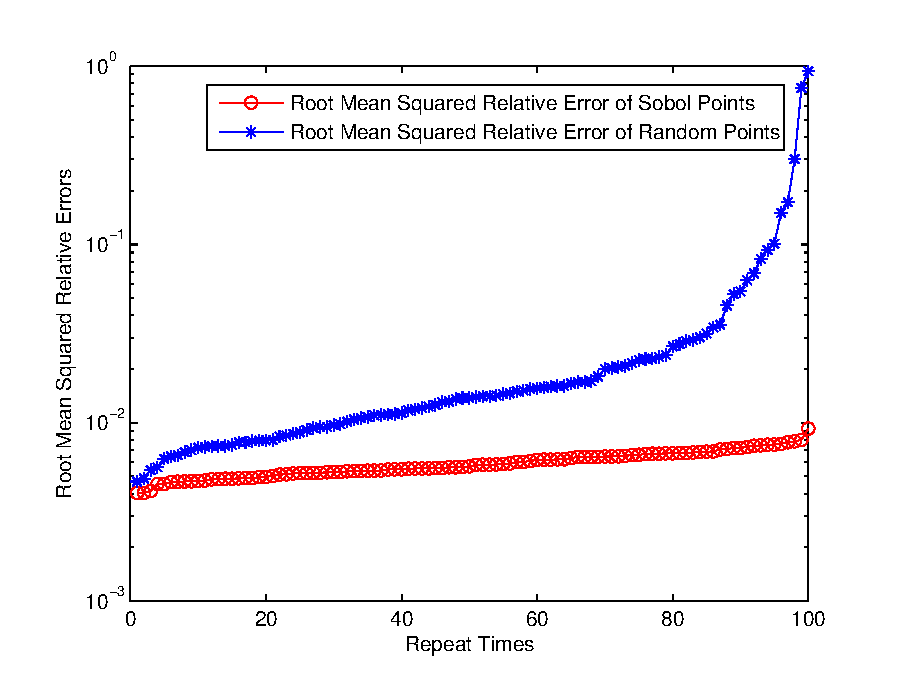
\includegraphics[width=6cm]{unilognormerror.eps}
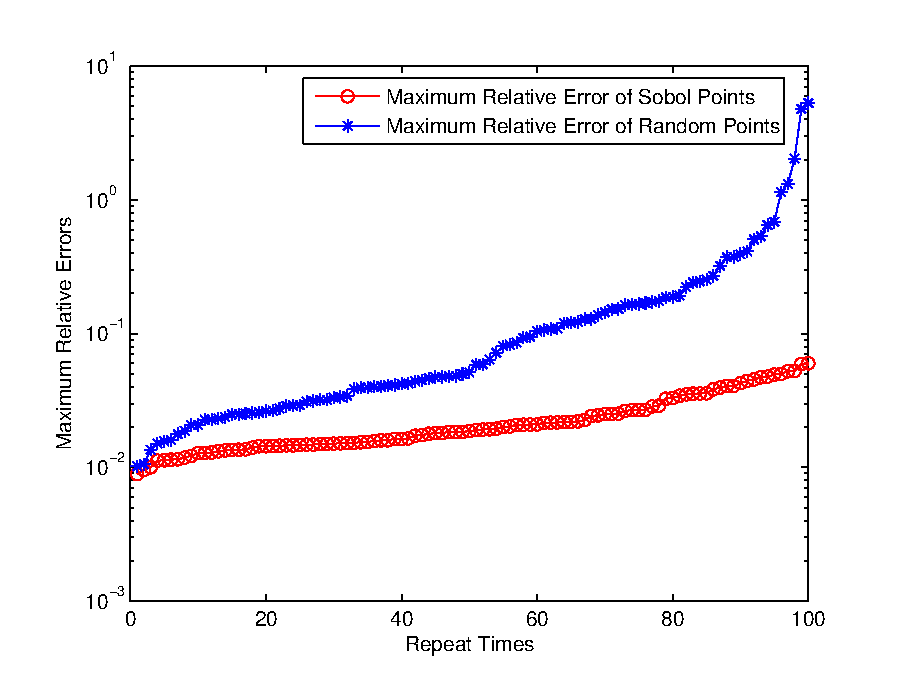
\includegraphics[width=6cm]{unilogsuperror.eps}
\caption{\label{fig:unierror} Relative Error Comparison between
Sobol Points and Random Points}
\end{center}
\end{figure}


Then, we tried a more complicated case with $d=2$. First, we choose
the univariate polynomials that is orthogonal under the inner
product, $\langle \boldsymbol{f},\boldsymbol{h}
\rangle=\int_{\Omega}\mathbf{L}_{\boldsymbol{x}}\boldsymbol{f}\left(\mathbf{L}_{\boldsymbol{x}}\boldsymbol{h}\right)^TdF_{\Omega}(\boldsymbol{x})$(REFERENCE!!).
Then, we use tensor product of these univariate polynomials to
construct multivariate polynomials up to degree $3$. We choose these
multivariate polynomials up to degree $3$ as our basis, and there
will be totally $10$ polynomials in the basis. Since compared to
univariate case, in this case, we only have polynomials up to degree
$3$, as a result, we choose a less fluctuant function,
$f(\boldsymbol{x})=4+e^{-0.7x_1-0.5x_2}\sin(0.3x_1+0.6x_2)$ as the
testing function. The same as in the univariate experiment, we use
$16$ sample points to estimate the regression coefficient
$\boldsymbol{\beta}$ in the model, and use $1000$ sample points to
test the model. We repeat the experiment $100$ times, and compute
both maximum of the relative error of the function value and the
relative root mean squared error of the function value. Figure
\ref{fig:mulerror} compares relative prediction errors in function
value between models using Sobol points, which is low discrepancy,
and models using simple random points. In the left plot, we compares
relative root mean squared errors in function value, while in the
right plot, we compares relative maximum errors in function value.
We conclude from \ref{fig:mulerror} that Sobol points work
substantially better than simple random points, and result in better
estimation of function values.

\begin{figure}[htpb]
\begin{center}
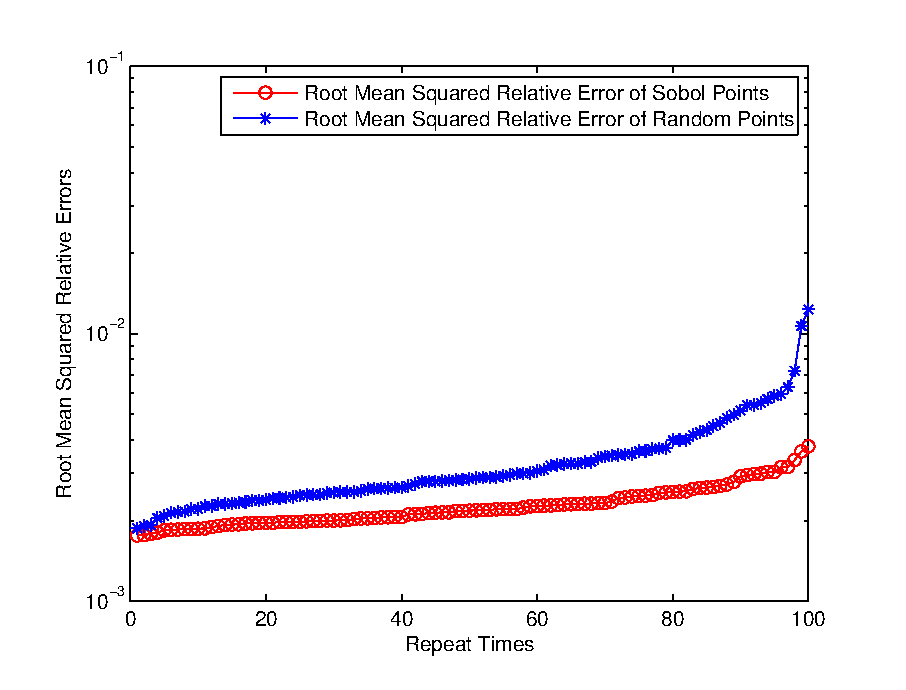
\includegraphics[width=6cm]{mullognormerror.eps}
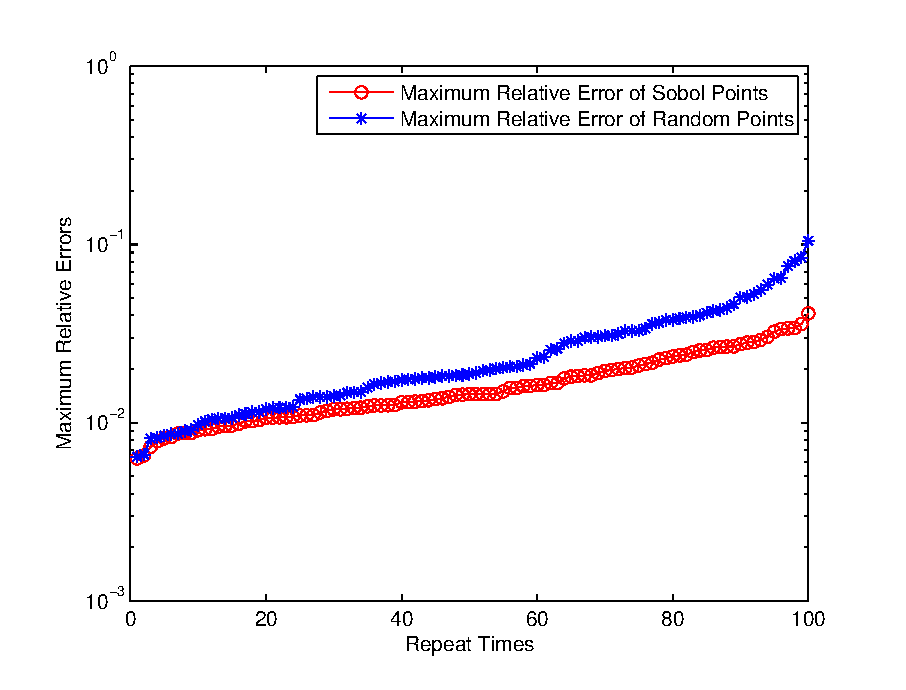
\includegraphics[width=6cm]{mullogsuperror.eps}
\caption{\label{fig:mulerror} Relative Error Comparison between
Sobol Points and Random Points}
\end{center}
\end{figure}

\section{Optimal Design When Gradient Information Is Available}
\subsection{D-optimality}
Continuous designs are represented by the measure $\xi$ over
$\Omega$, where $\Omega$ is the variable domain as defined
previously. If the design has $n$ trials at $n$ distinct points in
$\Omega$, we write:
$$\xi=\left\{\begin{array}{llll} \boldsymbol{x}_1\,\,&\boldsymbol{x}_2&\cdots&\boldsymbol{x}_n\\w_1\,\,&w_2&\cdots&w_n\end{array}\right\},$$
where $w_i$ is the weight on the sample point $\boldsymbol{x}_i$
with $0\leq w_i\leq 1$, for $i=1,\cdots,n$, and $\sum
\limits_{i=1}^n w_i=1$.

Optimal designs is a class of experimental designs that are optimal
with respect to some statistical criterion. In general, these
statistical criterion could be considered as minimizing some convex
function $\Psi\{\boldsymbol{M}(\xi)\}$, where $\boldsymbol{M}(\xi)$
is the information matrix, as defined in section $3$, and this
information matrix will depend on the design $\xi$. Many of the
design criteria are called by a letter of the alphabet, so this
large class of design criteria is sometimes called `alphabetic
optimality'. One of the most well-known `alphabetic optimality' is
D-optimality. By definition, a D-optimal design minimizes the
content of the confidence region, which is also the volume of the
ellipsoid, and this ellipsoid is defined as
$(\boldsymbol{\beta}-\hat{\boldsymbol{\beta}})^T\boldsymbol{G}^T\boldsymbol{G}(\boldsymbol{\beta}-\hat{\boldsymbol{\beta}})$.
It has been proved that D-optimality is equivalent to minimizing the
determinant of $\boldsymbol{M}^{-1}(\xi)$(REFERENCE), in which case,
we will have $\Psi\{\boldsymbol{M}(\xi)\}=-\log|\boldsymbol{M}|$.

Let the measure $\bar{\xi}$ put unit mass at the point
$\boldsymbol{x}$, then the derivative of $\Psi$ in the direction
$\bar{\xi}$ is defined as:
$$\phi(\boldsymbol{x},\xi)=\lim_{\alpha\rightarrow 0^+}\frac{1}{\alpha}\left[\Psi\{(1-\alpha)\boldsymbol{M}(\xi)+\alpha\boldsymbol{M}(\bar{\xi})\}-\Psi\{\boldsymbol{M}(\xi)\}\right].$$


Then, a well-known theorem, \textbf{The General Equivalence Theorem}
states the equivalence of the following three conditions on $\xi^*$:
\begin{enumerate}
\item The design $\xi^*$ minimizes $\Psi\{\boldsymbol{M}(\xi)\}$.
\item The design $\xi^*$ maximizes the minimum over $\Omega$ of
$\Phi(\boldsymbol{x},\xi)$.
\item The minimum over $\Omega$ of
$\Phi(\boldsymbol{x},\xi^*)=0$, the minimum occurring at the points
of support of the design.

As a consequence of $3$, we obtain the further condition:
\item For any non-optimum design $\xi$, the minimum over
$\Omega$ of $\Phi(\boldsymbol{x},\xi)<0$.
\end{enumerate}

By The General Equivalence Theorem, we could check whether a design
is optimal or not, and we could even find an optimal design over
$\Omega$.

\subsection{D-optimal Design When Gradient Information Is Available}
\label{section:Dopt}

A nature question to ask will be whether
gradient information will influence the optimal design? Our answer
is yes, and we discuss this upon the quadratic regression with
scalar variable, on interval $[-1,1]$, i.e $\Omega=[-1,1]$.

The classical model will be:
$$y_i=\boldsymbol{g}^T(x)\boldsymbol{\beta}+\varepsilon_i,$$
while, the model with gradient information will be:
$$\boldsymbol{y}_i=(\mathbf{L}_{x_i}\boldsymbol{g}^T)\boldsymbol{\beta}+\boldsymbol{\varepsilon}_i,\text{(Need more specified??write as a matrix??)}$$
where $\boldsymbol{g}(x)=(1,x,x^2)^T$, $\varepsilon_i$ are
independent and identically distributed random errors for classical
model with mean $0$ and variance $\sigma^2$, and
$\boldsymbol{\varepsilon}_i$ are independent and identically
distributed random errors for the model with gradient information,
with mean $0$ and covariance
$\sigma^2\widetilde{\boldsymbol{\Lambda}}$ as defined in section
\ref{section:statmodel}.

From the theory of optimal design, it is known that for classical
quadratic regression model, the derivative of $\Psi$ will be:
$$\Phi(x,\xi)=3-\boldsymbol{g}^T(x)\boldsymbol{M}(\xi)^{-1}\boldsymbol{g}(x),$$
where $3$ comes from the number of the terms in the basis, and as a
result, a D-optimal design will be(REFERENCE):
$$\xi^*=\left\{\begin{array}{lll}-1\,\,&0\,\,&1\\1/3\,\,&1/3\,\,&1/3\end{array}\right\}.$$
For the model with gradient information in univariate, given the
design $\xi$, it is obvious that:
$$\Phi(x,\xi)=3-\boldsymbol{g}^T(x)\boldsymbol{M}(\xi)^{-1}\boldsymbol{g}(x)-\lambda\boldsymbol{g}'(x)^T\boldsymbol{M}(\xi)^{-1}\boldsymbol{g}'(x),$$
with
$\boldsymbol{M}(\xi)=\frac{\sigma^2\boldsymbol{G}^T\boldsymbol{\Sigma}^{-1}\boldsymbol{G}}{m}=\sum\limits_{i=1}^nw_i\left(\boldsymbol{g}(x_i)\boldsymbol{g}^T(x_i)+\lambda\boldsymbol{g}'(x_i)
\left(\boldsymbol{g}'(x_i)\right)^T\right).$

Then, we will have the following theorem for the D-optimal design
with the univariate quadratic model involving gradient information.
\begin{thm}
For the univariate quadratic regression model with gradient
information defined above, a D-optimal design $\xi^*$ will be:

\begin{enumerate}
\item When $0\leq\lambda<\frac{\sqrt{65}-7}{8}$, $$\xi^*=\left\{\begin{array}{ccc}-1\,\,&0\,\,&1\\w\,\,&1-2w\,\,&w\end{array}\right\},$$
with
$w=\frac{1}{6}+\frac{1}{2}\lambda+\frac{1}{6}\sqrt{1+9\lambda+21\lambda^2}.$
\item When $\lambda>\frac{\sqrt{65}-7}{8}$, $$\xi^*=\left\{\begin{array}{ccc}-1\,\,&1\\ \frac{1}{2}\,\,&\frac{1}{2}\end{array}\right\}.$$
\end{enumerate}

\end{thm}
\begin{proof}
Suppose a D-optimal design is assumed to be:
$$\xi^*=\left\{\begin{array}{ccc}-1\,\,&0\,\,&1\\w\,\,&1-2w\,\,&w\end{array}\right\}.$$

It is obvious that $w\neq0$, since if $w=0$, $0$ will be the only
sample point, and the information matrix $\boldsymbol{M}(\xi)$ will
be singular.

Then, since
$\boldsymbol{M}(\xi)=\sum\limits_{i=1}^nw_i\left(\boldsymbol{g}(x_i)\boldsymbol{g}^T(x_i)+\lambda\boldsymbol{g}'(x_i)
\left(\boldsymbol{g}'(x_i)\right)^T\right)$, we will get,
$$\boldsymbol{M}(\xi^*)=\left(\begin{array}{ccc}1&0&2w\\0&2w+\lambda&0\\2w&0&w(2+8\lambda
)\end{array}\right).$$ Then,
$$\boldsymbol{M}^{-1}(\xi^*)=\left(\begin{array}{ccc}-\frac{1+4\lambda}{2w-1-4\lambda}&0&\frac{1}{2w-1-4\lambda}\\0&\frac{1}{2w+\lambda}&0\\\frac{1}{2w-1-4\lambda}&0&-\frac{1}{2(2w-1-4\lambda)w}\end{array}\right).$$
By
$\Phi(x,\xi)=3-\boldsymbol{g}^T(x)\boldsymbol{M}(\xi)^{-1}\boldsymbol{g}(x)-\lambda\boldsymbol{g}'(x)^T\boldsymbol{M}(\xi)^{-1}\boldsymbol{g}'(x)$,
we will have
\begin{eqnarray*}
\Phi(x,\xi^*)&=&\frac{1}{2(2w-1-4\lambda)w}x^4+\left(\frac{2\lambda}{(2w-1-4\lambda)w}-\frac{2}{2w-1-4\lambda}-\frac{1}{2w+\lambda}\right)x^2\\
&&+3-\frac{\lambda}{2w+\lambda}+\frac{1+4\lambda}{2w-1-4\lambda}.
\end{eqnarray*}

As $2w-1\leq0$, $w>0$, and $\lambda\geq0$, $\Phi(x,\xi^*)$ is a
parabola of $x^2$ with the coefficient of $x^4$,
$\frac{1}{2(2w-1-4\lambda)w}<0$. As a result, the minimum of
$\Phi(x,\xi^*)$ can only occurs when $x^2=0$ or $x^2=1$.

When $x^2=0$,
$$\Phi(0,\xi^*)=\frac{12w^2-4w-12w\lambda-\lambda-4\lambda^2}{(2w+\lambda)(2w-1-4\lambda)}=\frac{(w-w_{0+})(w-w_{0-})}{(2w+\lambda)(2w-1-4\lambda)},$$
where
$w_{0+}=\frac{1}{6}+\frac{1}{2}\lambda+\frac{1}{6}\sqrt{1+9\lambda+21\lambda^2}$,
and
$w_{0-}=\frac{1}{6}+\frac{1}{2}\lambda-\frac{1}{6}\sqrt{1+9\lambda+21\lambda^2}\leq0$,
when $\lambda\geq0$. It is obvious that
$(2w+\lambda)(2w-1-4\lambda)<0$.

When $x^2=1$,
\begin{eqnarray*}
\Phi(\pm1,\xi^*)&=&\frac{24w^3-8w^2-32w^2\lambda+10w\lambda+4\lambda^2-12w^2+4w+\lambda}{2(2w+\lambda)(2w-1-4\lambda)w}\\
&=&\frac{(w-\frac{1}{2})(w-w_{0+})(w-w_{0-})}{(2w+\lambda)(2w-1-4\lambda)w}
\end{eqnarray*}
It is obvious that $(2w+\lambda)(2w-1-4\lambda)w<0$.

\begin{enumerate}
\item When $0\leq\lambda\leq\frac{\sqrt{65}-7}{8}$, from simple
calculation, we will get
$$0<w_{0+}=\frac{1}{6}+\frac{1}{2}\lambda+\frac{1}{6}\sqrt{1+9\lambda+21\lambda^2}\leq\frac{1}{2}.$$
The design,
$$\xi^*=\left\{\begin{array}{ccc}-1\,\,&0\,\,&1\\w\,\,&1-2w\,\,&w\end{array}\right\},$$
with
$w=\frac{1}{6}+\frac{1}{2}\lambda+\frac{1}{6}\sqrt{1+9\lambda+21\lambda^2},$
will make $\Phi(0,\xi^*)=0$, and $\Phi(\pm1,\xi^*)=0$, which means
when $x\in[-1,1]$, $\Phi(x,\xi^*)\geq0$, thus, by The General
Equivalence Theorem, $\xi^*$ is a D-optimal design.

What's more, if $w=\frac{1}{2}$, we will get $\Phi(0,\xi^*)<0$,
which means $$\xi=\left\{\begin{array}{ccc}-1\,\,&1\\
\frac{1}{2}\,\,&\frac{1}{2}\end{array}\right\}$$ could not be a
D-optimal design.

\item When $\lambda>\frac{\sqrt{65}-7}{8}$, the design
$$\xi^*=\left\{\begin{array}{ccc}-1\,\,&1\\ \frac{1}{2}\,\,&\frac{1}{2}\end{array}\right\}$$
will make $\Phi(0,\xi^*)>0$, and $\Phi(\pm1,\xi^*)=0$, which means
when $x\in[-1,1]$, $\Phi(x,\xi^*)\geq0$, thus, by The General
Equivalence Theorem, $\xi^*$ is a D-optimal design.
\end{enumerate}
\end{proof}

\begin{figure}[htpb]
\begin{center}
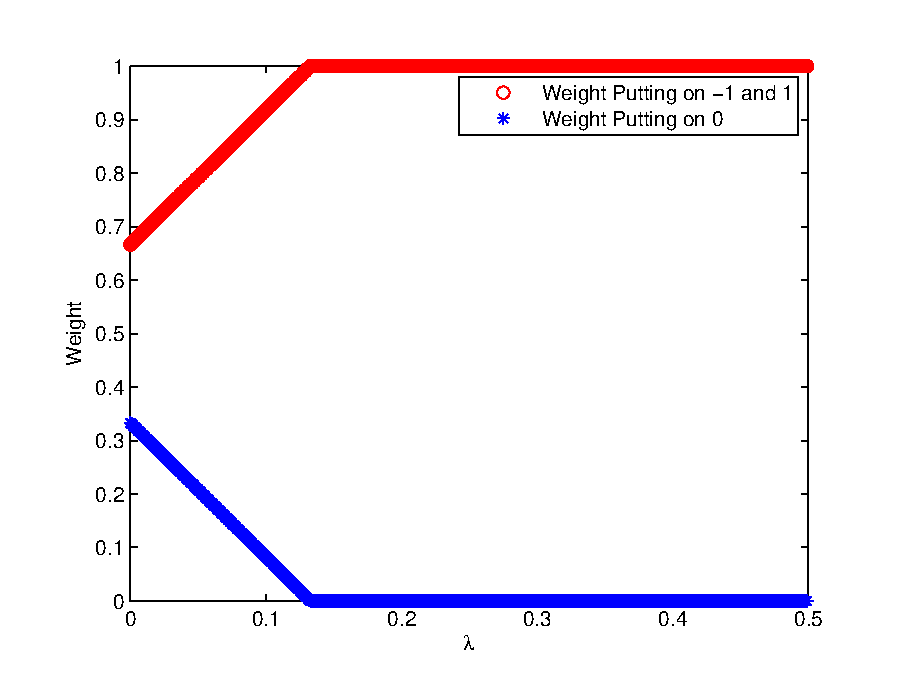
\includegraphics[width=8cm]{Dopt.eps}
\caption{\label{fig:DoptS} D Optimal Design Design Corresponding to
the Change of $\lambda$ }
\end{center}
\end{figure}

\subsection{I-optimal Design When Gradient Information Is Available}
Now, we will define an optimality criteria that corresponding to the
scaled integrated mean squared error defined in section
\ref{section:Iopt}, for which the optimal design minimizes the
scaled integrated mean squared error. We will call this optimality
criteria I optimality, since it is analogous to classical I
optimality without gradient information(REFERENCE). In this case, as
proved in proposition \ref{prop:Iopt}, we will have
$\Psi\{\boldsymbol{M}(\xi)\}=\tr(\boldsymbol{M}^{-1}(\xi)\boldsymbol{A})$,
where as defined in section \ref{section:Iopt},
$\boldsymbol{A}=\left(\langle Tg_i,Tg_j\rangle_{\mathcal
{L}_{2,F}^s(\Omega)}\right)_{i,j=1}^{m(d+1)}$.

\begin{pro}
\label{prop:Ider}
For I-optimality, the derivative of $\Psi$ will
be:
\begin{enumerate}
\item for the classical model without gradient information:
$$y_i=\boldsymbol{g}^T(x)\boldsymbol{\beta}+\varepsilon_i,$$
where $\varepsilon_i$ are independent and identically distributed
random errors for classical model with mean $0$ and variance
$\sigma^2$.
$$\Phi(\boldsymbol{x},\xi)=\tr(\boldsymbol{M}^{-1}(\xi)\boldsymbol{A})-\boldsymbol{g}^T(\boldsymbol{x})\boldsymbol{M}^{-1}(\xi)\boldsymbol{A}\boldsymbol{M}^{-1}(\xi)\boldsymbol{g}(\boldsymbol{x})$$


\item for the model with gradient information:
$$\boldsymbol{y}_i=(\mathbf{L}_{x_i}\boldsymbol{g}^T)\boldsymbol{\beta}+\boldsymbol{\varepsilon}_i,$$
where $\boldsymbol{\varepsilon}_i$ are independent and identically
distributed random errors for the model with gradient information,
with mean $0$ and covariance
$\sigma^2\widetilde{\boldsymbol{\Lambda}}$ as defined in section
\ref{section:statmodel}.
\begin{eqnarray*}
\Phi(x,\xi)&=&\tr(\boldsymbol{M}^{-1}(\xi)\boldsymbol{A})-\boldsymbol{g}^T(\boldsymbol{x})\boldsymbol{M}^{-1}(\xi)\boldsymbol{A}\boldsymbol{M}^{-1}(\xi)\boldsymbol{g}(\boldsymbol{x})\\
&&-\sum_{i=1}^d\lambda_i\left(\frac{\partial\boldsymbol{g}}{\partial
x_i}\right)^T(\boldsymbol{x})\boldsymbol{M}^{-1}(\xi)\boldsymbol{A}\boldsymbol{M}^{-1}(\xi)\frac{\partial\boldsymbol{g}}{\partial
x_i}(\boldsymbol{x})\\
\end{eqnarray*}
\end{enumerate}
\end{pro}

\begin{proof}
First, we compute the G\^{a}teaux derivative of $\Psi$ at
$\boldsymbol{M}_1$ in the direction of $\boldsymbol{M}_2$, which is
defined as:
$$G_{\Psi}(\boldsymbol{M}_1,\boldsymbol{M}_2)=\lim_{\varepsilon\rightarrow0^+}\frac{1}{\varepsilon}\left\{\Psi(\boldsymbol{M}_1+\varepsilon\boldsymbol{M}_2)-\Psi(\boldsymbol{M}_1)\right\}.$$
\begin{eqnarray*}
G_{\Psi}(\boldsymbol{M}_1,\boldsymbol{M}_2) &=&
\lim_{\varepsilon\rightarrow0^+}\frac{1}{\varepsilon}\{\tr[(\boldsymbol{M}_1+\varepsilon\boldsymbol{M}_2)^{-1}\boldsymbol{A}]-\tr(\boldsymbol{M}_1^{-1}\boldsymbol{A})\}\\
&=&
\lim_{\varepsilon\rightarrow0^+}\frac{1}{\varepsilon}\{\tr[((\boldsymbol{M}_1+\varepsilon\boldsymbol{M}_2)^{-1}+\boldsymbol{M}_1^{-1})\boldsymbol{A}]\}\\
&=&
\lim_{\varepsilon\rightarrow0^+}\frac{1}{\varepsilon}\{\tr[((I+\varepsilon\boldsymbol{M}_1^{-1}\boldsymbol{M}_2)^{-1}\boldsymbol{M}_1^{-1}-\boldsymbol{M}_1^{-1})\boldsymbol{A}]\}\\
&=&
\lim_{\varepsilon\rightarrow0^+}\frac{1}{\varepsilon}\{\tr[((I-\varepsilon\boldsymbol{M}_1^{-1}\boldsymbol{M}_2+\mathcal{O}(\varepsilon^2))\boldsymbol{M}_1^{-1}-\boldsymbol{M}_1^{-1})\boldsymbol{A}]\}\\
&=&
\lim_{\varepsilon\rightarrow0^+}\frac{1}{\varepsilon}\{\tr(-\varepsilon\boldsymbol{M}_1^{-1}\boldsymbol{M}_2\boldsymbol{M}_1^{-1}\boldsymbol{A})+\mathcal{O}(\varepsilon^2)\}\\
&=&
-\tr(\boldsymbol{M}_1^{-1}\boldsymbol{M}_2\boldsymbol{M}_1^{-1}\boldsymbol{A})
\end{eqnarray*}

Then, we will compute the Fr\'{e}chet derivative of $\Psi$ at
$\boldsymbol{M}_1$ in the direction of $\boldsymbol{M}_2$, which is
defined as:
$$F_{\Psi}(\boldsymbol{M}_1,\boldsymbol{M}_2)=\lim_{\varepsilon\rightarrow0^+}\frac{1}{\varepsilon}\left\{\Psi((1-\varepsilon)\boldsymbol{M}_1+\varepsilon\boldsymbol{M}_2)-\Psi(\boldsymbol{M}_1)\right\}.$$
Since it is easy to show that
$F_{\Psi}(\boldsymbol{M}_1,\boldsymbol{M}_2)=G_{\Psi}(\boldsymbol{M}_1,\boldsymbol{M}_2-\boldsymbol{M}_1)$,
we will get,
\begin{eqnarray*}
F_{\Psi}(\boldsymbol{M}_1,\boldsymbol{M}_2)&=&-\tr[(\boldsymbol{M}_1^{-1}\boldsymbol{M}_2\boldsymbol{M}_1^{-1}-\boldsymbol{M}_1^{-1})\boldsymbol{A}]\\
&=&-\tr(\boldsymbol{M}_1^{-1}\boldsymbol{M}_2\boldsymbol{M}_1^{-1}\boldsymbol{A})+\tr(\boldsymbol{M}^{-1}_1\boldsymbol{A})\\
&=&
-\tr(\boldsymbol{M}_2\boldsymbol{M}_1^{-1}\boldsymbol{A}\boldsymbol{M}_1^{-1})+\tr(\boldsymbol{M}^{-1}_1\boldsymbol{A})
\end{eqnarray*}

Since
$\Phi(\boldsymbol{x},\xi)=F_{\Psi}(\boldsymbol{M}(\xi),\boldsymbol{M}(\bar{\xi}))$,
where $\bar{\xi}$ put unit mass at the point $\boldsymbol{x}$, from
simple calculation, we will have,
\begin{enumerate}
\item for the classical model without gradient information:
$$\Phi(\boldsymbol{x},\xi)=F_{\Psi}(\boldsymbol{M}(\xi),\boldsymbol{g}(\boldsymbol{x})\boldsymbol{g}^T(\boldsymbol{x}))=\tr(\boldsymbol{M}^{-1}(\xi)\boldsymbol{A})-\boldsymbol{g}^T(\boldsymbol{x})\boldsymbol{M}^{-1}(\xi)\boldsymbol{A}\boldsymbol{M}^{-1}(\xi)\boldsymbol{g}(\boldsymbol{x})$$


\item for the model with gradient information:
\begin{eqnarray*}
\Phi(x,\xi)&=&F_{\Psi}\left(\boldsymbol{M}(\xi),\boldsymbol{g}(\boldsymbol{x})\boldsymbol{g}^T(\boldsymbol{x})+\sum_{i=1}^d\lambda_i(\boldsymbol{x})\frac{\partial\boldsymbol{g}}{\partial
x_i}(\boldsymbol{x})\left(\frac{\partial\boldsymbol{g}}{\partial
x_i}\right)^T\right)\\
&=&\tr(\boldsymbol{M}^{-1}(\xi)\boldsymbol{A})-\boldsymbol{g}^T(\boldsymbol{x})\boldsymbol{M}^{-1}(\xi)\boldsymbol{A}\boldsymbol{M}^{-1}(\xi)\boldsymbol{g}(\boldsymbol{x})\\
&&-\sum_{i=1}^d\lambda_i\left(\frac{\partial\boldsymbol{g}}{\partial
x_i}\right)^T(\boldsymbol{x})\boldsymbol{M}^{-1}(\xi)\boldsymbol{A}\boldsymbol{M}^{-1}(\xi)\frac{\partial\boldsymbol{g}}{\partial
x_i}(\boldsymbol{x})\\
\end{eqnarray*}
\end{enumerate}
\end{proof}

Then, as the same in section \ref{section:Dopt}, we will discuss
upon the quadratic regression with scalar variable, on interval
$[-1,1]$, i.e $\Omega=[-1,1]$. For simplicity, in the following
discussion, we will define $Tf=f$, then
$\boldsymbol{A}=\int_{\Omega}\boldsymbol{g}(\boldsymbol{x})\boldsymbol{g}^T(\boldsymbol{x})dF_P(\boldsymbol{x})$.
In general, we could have $T$ to be any linear and bounded operator,
and as long as it is determined, we could always find an I optimal
design corresponding to a particular $T$.

The classical model will be:
$$y_i=\boldsymbol{g}^T(x)\boldsymbol{\beta}+\varepsilon_i,$$
while, the model with gradient information will be:
$$\boldsymbol{y}_i=(\mathbf{L}_{x_i}\boldsymbol{g}^T)\boldsymbol{\beta}+\boldsymbol{\varepsilon}_i,\text{(Need more specified??write as a matrix??)}$$
where $\boldsymbol{g}(x)=(1,x,x^2)^T$, $\varepsilon_i$ are
independent and identically distributed random errors for classical
model with mean $0$ and variance $\sigma^2$, and
$\boldsymbol{\varepsilon}_i$ are independent and identically
distributed random errors for the model with gradient information,
with mean $0$ and covariance
$\sigma^2\widetilde{\boldsymbol{\Lambda}}$ as defined in section
\ref{section:statmodel}.

For the classical quadratic regression model, as proved in
proposition \ref{prop:Ider}, we have,
$$\Phi(x,\xi)=\tr\left(\boldsymbol{M}^{-1}(\xi)\boldsymbol{A}\right)-\boldsymbol{g}^T(x)\boldsymbol{M}^{-1}(\xi)\boldsymbol{A}\boldsymbol{M}^{-1}(\xi)\boldsymbol{g}(x).$$
It is easy to prove by the $3$rd condition of the General
Equivalence Theorem that the design:
$$\xi^*=\left\{\begin{array}{ccc}-1\,\,&0\,\,&1\\1/4\,\,&1/2\,\,&1/4\end{array}\right\}$$
is an I optimal design.

For the model with gradient information in univariate, given the
design $\xi$, as proved in proposition \ref{prop:Ider}, we have,
$$\Phi(x,\xi)=\tr\left(\boldsymbol{M}^{-1}(\xi)\boldsymbol{A}\right)-\boldsymbol{g}^T(x)\boldsymbol{M}^{-1}(\xi)\boldsymbol{A}\boldsymbol{M}^{-1}(\xi)\boldsymbol{g}(x)-\lambda\boldsymbol{g}'(x)^T\boldsymbol{M}^{-1}(\xi)\boldsymbol{A}\boldsymbol{M}^{-1}(\xi)\boldsymbol{g}'(x).$$

Then, we will have the following theorem for the I optimal design
with univariate quadratic model involving gradient information.

\begin{thm}
For the univariate quadratic regression model with gradient
information defined above, we will have an I optimal design $\xi^*$,
$$\xi^*=\left\{\begin{array}{ccc}-1\,\,&0\,\,&1\\w\,\,&1-2w\,\,&w\end{array}\right\},$$
with $w$ is the root that lies in $[0,0.5]$ of the $p(w)$, which is
a polynomial of degree $4$,\small
$$960w^4\lambda+\left(128+960\lambda^2+400\lambda\right)w^3+\left(240\lambda^3-300\lambda^2-160\lambda-32\right)w^2-\left(36\lambda^2+12\lambda\right)w-\left(3\lambda^2+12\lambda^3\right).$$\normalsize
Later in the proof, we will demonstrate numerically that there will
be such a solution that lies in $[0,0.5]$.
\end{thm}
\begin{proof}
As given,
$$\xi^*=\left\{\begin{array}{ccc}-1\,\,&0\,\,&1\\w\,\,&1-2w\,\,&w\end{array}\right\},$$
it is obvious that $w\neq0$, since if $w=0$, $0$ will be the only
sample point, and the information matrix $\boldsymbol{M}(\xi)$ will
be singular.

Then, since
$\boldsymbol{M}(\xi)=\sum\limits_{i=1}^nw_i\left(\boldsymbol{g}(x_i)\boldsymbol{g}^T(x_i)+\lambda\boldsymbol{g}'(x_i)
\left(\boldsymbol{g}'(x_i)\right)^T\right)$, we will get,
$$\boldsymbol{M}(\xi^*)=\left(\begin{array}{ccc}1&0&2w\\0&2w+\lambda&0\\2w&0&w(2+8\lambda
)\end{array}\right).$$ Then,
$$\boldsymbol{M}^{-1}(\xi^*)=\left(\begin{array}{ccc}-\frac{1+4\lambda}{2w-1-4\lambda}&0&\frac{1}{2w-1-4\lambda}\\0&\frac{1}{2w+\lambda}&0\\\frac{1}{2w-1-4\lambda}&0&-\frac{1}{2(2w-1-4\lambda)w}\end{array}\right).$$

Since
$\boldsymbol{A}=\int_{\Omega}\boldsymbol{g}(x)\boldsymbol{g}^T(x)dF_P(x)$,
and $\boldsymbol{g}(x)=(1,x,x^2)^T$, we will have,
$$\boldsymbol{A}=\frac{1}{2}\int_{-1}^1\boldsymbol{g}(x)\boldsymbol{g}^T(x)dx=\frac{1}{2}\int_{-1}^1\left(\begin{array}{ccc}1&x&x^2\\x&x^2&x^3\\x^2&x^3&x^4\end{array}\right)dx=\left(\begin{array}{ccc}1&0&\frac{1}{3}\\0&\frac{1}{3}&0\\\frac{1}{3}&0&\frac{1}{5}\end{array}\right).$$

As a result,
\begin{eqnarray*}
\tr\left(\boldsymbol{M}^{-1}\boldsymbol{A}\right)&=&\tr\left(\begin{array}{ccc}-\frac{2(1+6\lambda)}{3(2w-4\lambda-1)}&0&-\frac{2(1+10\lambda)}{15(2w-4\lambda-1)}\\0&\frac{1}{3(2w+\lambda)}&0\\
\frac{6w-1}{6w(2w-4\lambda-1)}&0&\frac{10w-3}{30w(2w-4\lambda-1)}\end{array}\right)\\
&=&-\frac{240\lambda
w^2+(120\lambda^2+50\lambda+16)w+3\lambda}{30(2w-4\lambda-1)(2w+\lambda)w}
\end{eqnarray*}

As a result, we will get,
\begin{eqnarray*}
&&\Phi(x,\xi^*)\\
&=&\tr\left(\boldsymbol{M}^{-1}(\xi)\boldsymbol{A}\right)-\boldsymbol{g}^T(x)\boldsymbol{M}^{-1}(\xi)\boldsymbol{A}\boldsymbol{M}^{-1}(\xi)\boldsymbol{g}(x)-\lambda\boldsymbol{g}'(x)^T\boldsymbol{M}^{-1}(\xi)\boldsymbol{A}\boldsymbol{M}^{-1}(\xi)\boldsymbol{g}'(x)\\
&=&
-\frac{1}{60(2w-4\lambda-1)^2(2w+\lambda)^2w^2}\left(Coef_2x^4+Coef_1x^2+Coef_0\right)
\end{eqnarray*}
where
$$Coef_2=240w^4+(240\lambda-80)w^3+\left(60\lambda^2-80\lambda+12\right)w^2-\left(20\lambda^2-12\lambda\right)w+3\lambda^2,$$
\begin{eqnarray*}
Coef_1&=&(-960\lambda-240)w^4+\left(-960\lambda^2-640\lambda-48\right)w^3+\left(-240\lambda^3+240\lambda^2+240\lambda+20\right)w^2\\
&&+56\lambda^2w+12\lambda^3
\end{eqnarray*}
and
\begin{eqnarray*}
Coef_0&=&1920\lambda
w^5+\left(1920\lambda^2+800\lambda+256\right)w^4+\left(480\lambda^3-600\lambda^2-320\lambda-64\right)w^3\\
&&-\left(72\lambda^2+24\lambda\right)w^2-\left(24\lambda^3+6\lambda^2\right)w.
\end{eqnarray*}

It is easy to prove that,
\begin{eqnarray*}
Coef_2&=&240w^4+(240\lambda-80)w^3+\left(60\lambda^2-80\lambda+12\right)w^2-\left(20\lambda^2-12\lambda\right)w+3\lambda^2\\
&=& \left(60w^2-20w+3\right)(2w+\lambda)^2\\
&=&
\left(60\left(w-\frac{1}{6}\right)^2+\frac{4}{3}\right)(2w+\lambda)^2>0.
\end{eqnarray*}

As a result, it is obvious that $\Phi(x,\xi^*)$ is a parabola of
$x^2$ with the coefficient of $x^4$ being negative. Then, the
minimum of $\Phi(x,\xi^*)$ can only occur when $x^2=0$ or $x^2=1$.

When $x^2=0$,
$$\Phi(0,\xi^*)=-\frac{p(w)}{30(2w-4\lambda-1)^2(2w+\lambda)^2w},$$
where
$p(w)=960w^4\lambda+\left(128+960\lambda^2+400\lambda\right)w^3+\left(240\lambda^3-300\lambda^2-160\lambda-32\right)w^2-\left(36\lambda^2+12\lambda\right)w-\left(3\lambda^2+12\lambda^3\right)$.

When $x^2=1$,
$$\Phi(0,\xi^*)=-\frac{\left(w-\frac{1}{2}\right)p(w)}{30(2w-4\lambda-1)^2(2w+\lambda)^2w^2}.$$

It would be easy to check that when $w=\frac{1}{2}$,
$\Phi(0,\xi^*)=-\frac{48\lambda^3+24\lambda^2+64\lambda+8}{30(2w-4\lambda-1)^2(2w+\lambda)^2w}$,
which is always negative when $\lambda\geq 0$ and $w>0$, and this
means that
$$\xi^*=\left\{\begin{array}{ccc}-1\,\,&1\\
\frac{1}{2}\,\,&\frac{1}{2}\end{array}\right\}$$ can not be an
I-optimal design.

As a result, an I-optimal design $\xi^*$ will be, $\xi^*$,
$$\xi^*=\left\{\begin{array}{ccc}-1\,\,&0\,\,&1\\w\,\,&1-2w\,\,&w\end{array}\right\},$$
with $w$ is the root that lies in $[0,0.5]$ of the $p(w)$, which is
a polynomial of degree $4$,
$p(w)=960w^4\lambda+\left(128+960\lambda^2+400\lambda\right)w^3+\left(240\lambda^3-300\lambda^2-160\lambda-32\right)w^2-\left(36\lambda^2+12\lambda\right)w-\left(3\lambda^2+12\lambda^3\right).$

Now, let's look at the numerical result of the I-optimal design done
by Matlab , with $\lambda$ varying from $0$ to $99999$, which in
application $99999$ for $\lambda$ is far large enough.
\begin{figure}[htpb]
\begin{center}
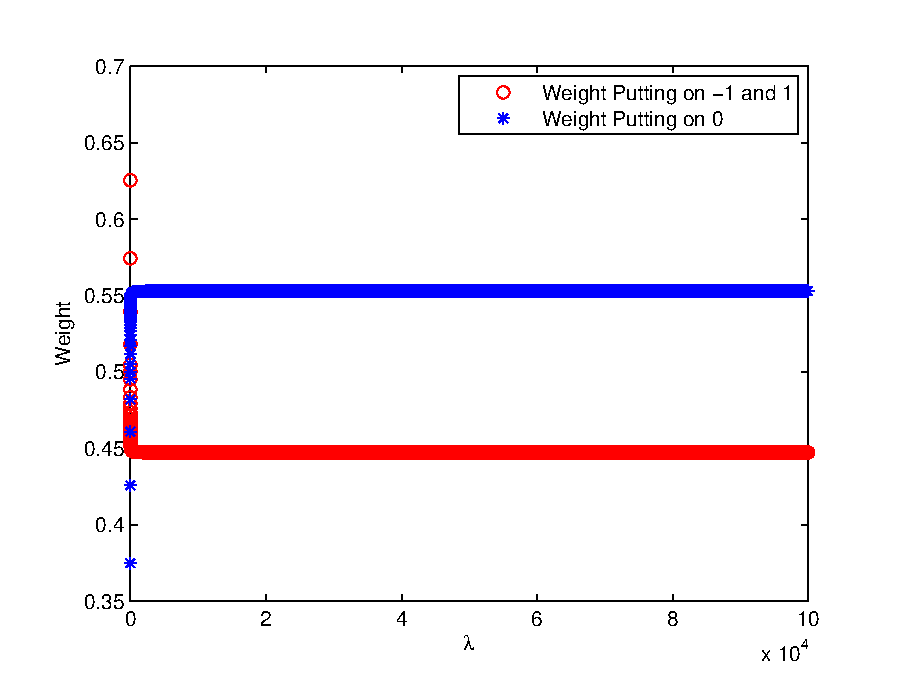
\includegraphics[width=8cm]{IoptL.eps}
\caption{\label{fig:IoptL} I Optimal Design Design Corresponding to
the Change of $\lambda$, $\lambda\in[0,99999]$ }
\end{center}
\end{figure}

\begin{figure}[htpb]
\begin{center}
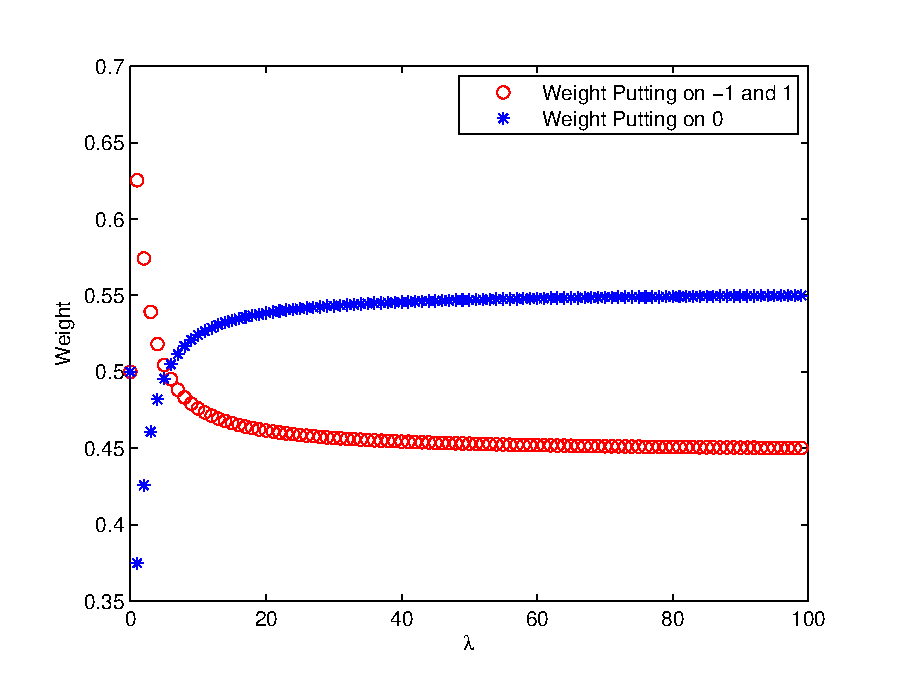
\includegraphics[width=8cm]{IoptM.eps}
\caption{\label{fig:IoptM} I Optimal Design Design Corresponding to
the Change of $\lambda$, $\lambda\in[0,99]$ }
\end{center}
\end{figure}

\begin{figure}[htpb]
\begin{center}
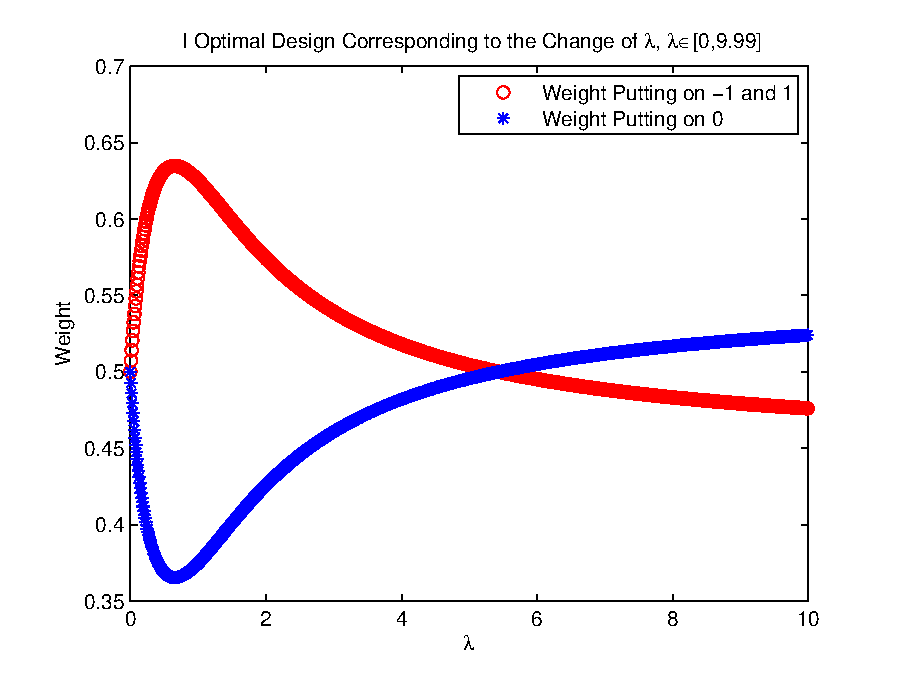
\includegraphics[width=8cm]{IoptS.eps}
\caption{\label{fig:IoptS} I Optimal Design Design Corresponding to
the Change of $\lambda$, $\lambda\in[0,9.99]$ }
\end{center}
\end{figure}

We could see from figure \ref{fig:IoptL} and the numerical result,
by the continuity of the root of $p(w)$ with respect to $\lambda$,
when $\lambda$ tends to be very large, the I optimal design will
tend to be stable, and will be very close to
$$\xi^*=\left\{\begin{array}{ccc}-1\,\,&0\,\,&1\\0.2236\,\,&0.5528\,\,&0.2236\end{array}\right\}.$$

From figure \ref{fig:IoptM} and figure \ref{fig:IoptS}, we could see
that when $\lambda=0$, the I optimal design will be
$$\xi^*=\left\{\begin{array}{ccc}-1\,\,&0\,\,&1\\1/4\,\,&1/2\,\,&1/4\end{array}\right\},$$
which is consistent with the I optimal design for the classical
model without gradient information. And, with $\lambda$ getting
large from $0$, the weight on $-1$ and $1$ first increases and
exceeds the weight on $0$, and then decreases and finally will keep
below the weight on $0$. Also, from the numerical result, when
$\lambda=1$, which means the variance of the function value and the
variance of the first derivative value is the same, we will have the
I optimal design as:












\end{proof}



%% The Appendices part is started with the command \appendix;
%% appendix sections are then done as normal sections
%% \appendix

%% \section{}
%% \label{}

%% References
%%
%% Following citation commands can be used in the body text:
%% Usage of \cite is as follows:
%%   \cite{key}          ==>>  [#]
%%   \cite[chap. 2]{key} ==>>  [#, chap. 2]
%%   \citet{key}         ==>>  Author [#]

%% References with bibTeX database:

\bibliographystyle{model1a-num-names}
\bibliography{<your-bib-database>}

%% Authors are advised to submit their bibtex database files. They are
%% requested to list a bibtex style file in the manuscript if they do
%% not want to use model1a-num-names.bst.

%% References without bibTeX database:

% \begin{thebibliography}{00}

%% \bibitem must have the following form:
%%   \bibitem{key}...
%%

% \bibitem{}

% \end{thebibliography}


\end{document}

%%
%% End of file `elsarticle-template-1a-num.tex'.
